\scanpage{10}

\uline{Condition f)} $\forall A\in F$, $A$ loc. fermé (i.e. $A=B-C$, $B,C\in F_0$) les comp. connexes de $A$ sont en nb fini (donc ouvertes dans $A$) et $\in F$.

\figure{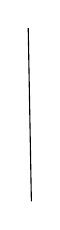
\begin{tikzpicture}\draw (0,2.2)--(.04,0);\end{tikzpicture}}

Cela implique donc que $A$ \inserted{loc. fermé, $\in F$} est connexe \unsure{ssi} \deleted{que} $\deleted{\unsure{B}}A',A''\in F$, $A'\cap A''=\varnothing$, $A'\cup A''=A$, $A'$ et $A''$ fermés ds $A$ (trace donc sur $A$ d'éléments de $F_0$), on a $A'=\varnothing$ ou $A''=\varnothing$ : c'est donc là une condition qui ne fait pas intervenir la top. de $X$, mais $F_0$ directement. De plus, \deleted{\unsure{on a} $(\varphi)$ si $A$ est loc. fermé}\inserted{$F_0$ satisfait} $(\varphi)$ $A=B-C$, avec $B,C\in F_0$, $C\subset B$, alors $A$ se décompose en réunion disjointe \uuline{finie} \unsure{d'éléments|d'élts} de $F$ \unsure{rel. ferm|rel. fermés} dans $A$ \inserted{(i.e. traces sur $A$ d'$\in$ de $F_0$)}, qui sont ainsi $F_0$-connexes. \deleted{C'est là une condition \inserted{\unsure{portant}} sur $F_0$).}

Si les ouverts $\in F$ forment une base de la top. de $X$, alors la condition f) (qui peut être considérée comme une condition sur l'ens de parties $F_0$) implique que les $A\in F$ (du moins ceux qui sont loc. fermés --- en fait cette restriction est inutile) sont \uline{loc. connexes}.

\mspage{11}
